\section{Case and Person Registry Design Rationale}

The TAC Industries application layer is underpinned by a deliberately minimal and structured data model designed to support investigative workflows while minimising unnecessary data collection. Rather than attempting to model a full law-enforcement records system, the platform focuses on two core registries: a case registry and a person registry.

The case registry acts as the administrative and operational anchor for all investigative activity. Each case record contains high-level metadata such as case type, status, owning bureau, and lifecycle timestamps. Evidence, intelligence submissions, and associated persons are linked to cases rather than stored independently, ensuring contextual integrity and reducing the risk of orphaned records.

The person registry is designed to store only individuals who are relevant to an active or historical case. Persons are linked to cases in defined roles, such as suspect, victim, witness, or reporting party, rather than existing as standalone profiles. This approach supports data minimisation and ensures that personal data is stored only where there is a clear investigative purpose.


\begin{figure}[!ht]
    \centering
    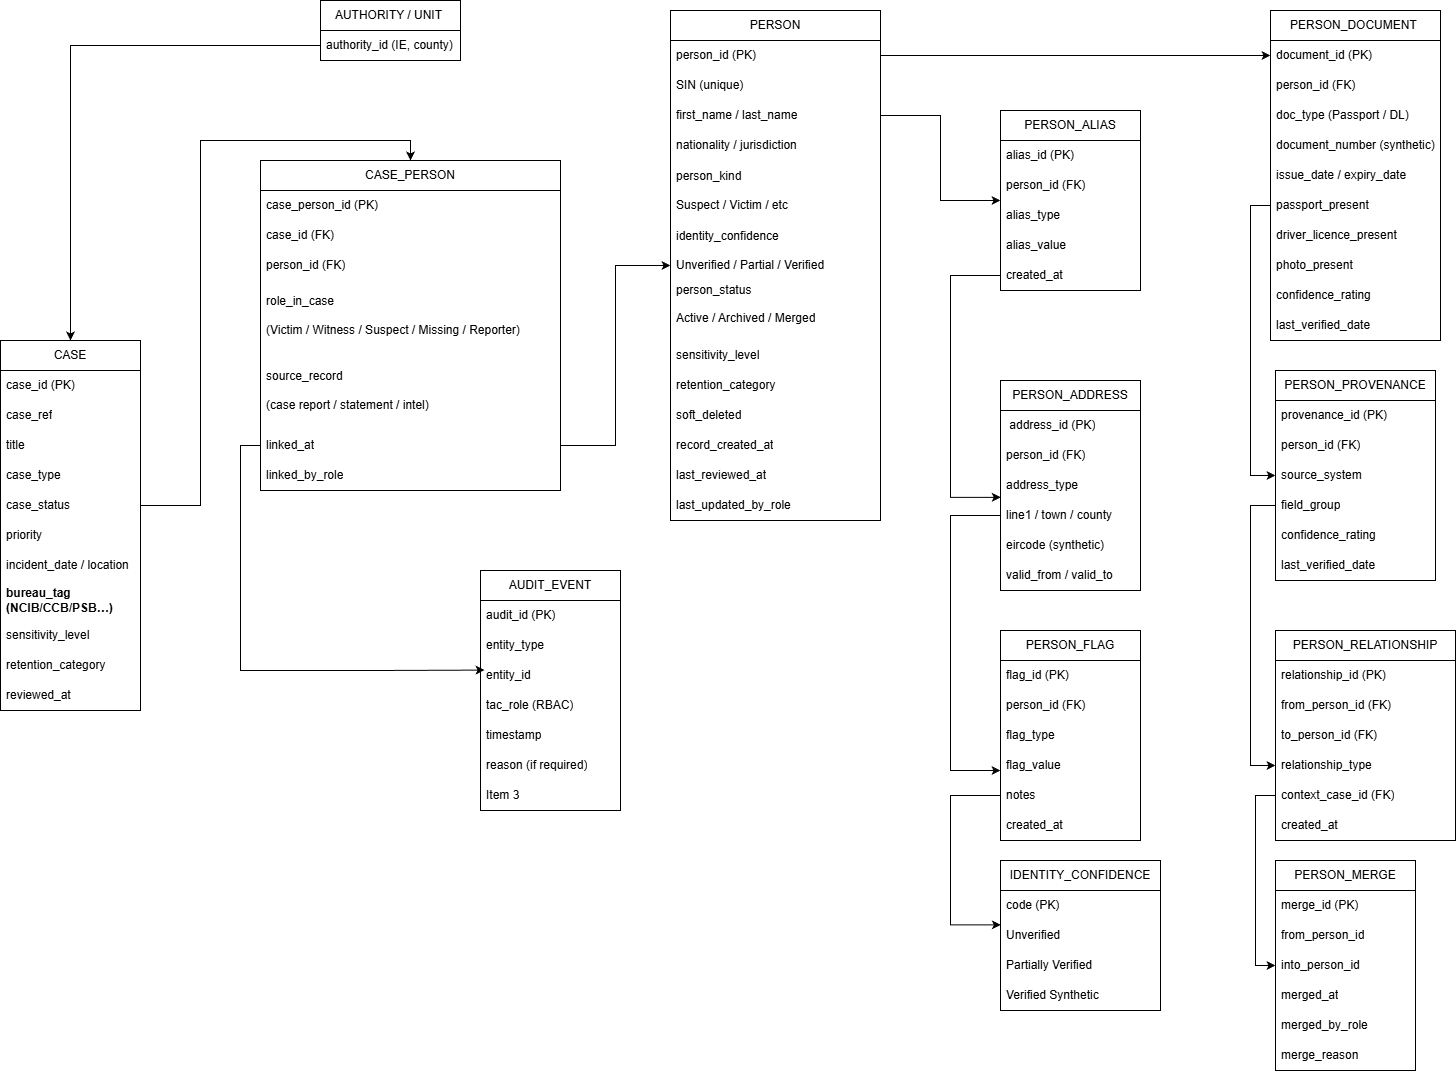
\includegraphics[width=\textwidth]{Images/ERD-Person-Case.png}
    \caption{TAC Industries logical network segmentation and infrastructure overview}
    \label{fig:network-architecture}
\end{figure}

\section{Identity Confidence and Synthetic Identities}

Given the academic nature of the project and the sensitivity of investigative data, TAC Industries operates exclusively on synthetic identities. All personal identifiers, documents, and attributes are artificially generated and do not correspond to real individuals.

To support realistic investigative workflows, the platform introduces the concept of identity confidence. Each person record is assigned a confidence level that reflects the degree to which the identity has been validated within the context of a case. Confidence levels range from unverified through partially verified to verified, allowing the system to represent uncertainty without making factual assertions.

\section{Audit, Provenance, and Data Lifecycle Controls}

Auditability and data governance are treated as first-class concerns within the TAC Industries data model. All significant actions affecting cases or person records are logged, including creation, modification, association, and lifecycle transitions. Audit records capture the action performed, the role responsible, and the timestamp, without exposing unnecessary personal information\cite{nist80092}.

Data provenance metadata is used to indicate the source and confidence of stored information. This allows users to distinguish between data derived from different investigative activities or synthetic generation processes and supports informed decision-making without overreliance on unverified inputs.

Lifecycle controls are incorporated to support responsible data handling. Records may be archived, merged, or soft-deleted rather than permanently removed, preserving historical integrity while respecting retention and governance principles\cite{gdpr2016}. These controls align the data model with data protection best practices and ensure that investigative records remain traceable and accountable over time.
